\documentclass[a4paper]{article}

%% Language and font encodings
\usepackage[english]{babel}
\usepackage[utf8x]{inputenc}
\usepackage[T1]{fontenc}

%% Sets page size and margins
\usepackage[a4paper,top=3cm,bottom=2cm,left=3cm,right=3cm,marginparwidth=2cm]{geometry}

%% Useful packages
\usepackage{algorithm}
\usepackage{amsfonts}
\usepackage{amsmath}
\usepackage{amssymb}
\usepackage{amsthm}
\usepackage{bbm}
\usepackage[colorinlistoftodos]{todonotes}
% \usepackage[colorlinks=true, allcolors=blue]{hyperref}
\usepackage{enumerate}
\usepackage{float}
\usepackage{graphicx}
\usepackage{mathrsfs}
\usepackage{pgfplots}
\usepackage{subcaption}
\usepackage{tikz}
\usepackage{tikzscale}
\usetikzlibrary{shapes.geometric, arrows}
\tikzset{
    vertex/.style={circle,draw,minimum size=1.5em},
    edge/.style={->,> = latex'}
}
\tikzstyle{triger} = [circle, minimum width=2cm, minimum height=1cm, text centered, draw=black]
\tikzstyle{process} = [rectangle, minimum width=1cm, minimum height=1cm, text centered, draw=black]
\tikzstyle{decision} = [diamond, minimum width=2cm, minimum height=1cm, text centered, draw=black]
\tikzstyle{block} = [rectangle, minimum width=3cm, minimum height=3cm, text centered, draw=black]
\tikzstyle{arrow} = [thick,->,>=stealth]
\pgfplotsset{compat=1.18} 

\title{Midterm}
\author{Kevin Chang}

\newtheorem{definition}{Definition}
\newtheorem{problem}{Problem}
\newtheorem{property}{Property}[section]
\newtheorem{theorem}{Theorem}[section]
\newtheorem{suspect}{Suspect}[section]
\newtheorem{example}{Example}
\newtheorem{lemma}[theorem]{Lemma}

\graphicspath{ {./images/} }

\begin{document}
\maketitle

\section{}
Suppose we’d like to build a classification rule for a finite population $\Omega$ of pairs $(x_i , y_i)$ where $x_i$ are integers and $y_i$ are assumed to be in $\{-1, 1\}$.
Let $n$ denote the size of $\Omega$.
\begin{enumerate}[(i)]
    \item Compute the function $\hat{y}_\mathit{me}(x)$ that minimizes the number of classification errors on this population.

The function that minimizes the number of classification errors (majority vote) is
$$\hat{y}_{\mathrm{me}}(x) = \operatorname{sign}\!\Big(\sum_{i \in \Omega} \mathbbm{1}(x_i = x)\, y_i \Big)$$
(with arbitrary tie-breaking when the sum is zero).  
The minimal empirical error rate is
$$\frac{1}{n} \sum_{x \in \Omega} \min(n_x^+, n_x^-),$$
where $n_x^+ = |\{ x_i \in \Omega \wedge x_i = x : y_i = 1 \}|$ and $n_x^- = |\{ x_i \in \Omega \wedge x_i = x : y_i = -1 \}|$.

    \item Suppose we instead choose to minimize the square-loss over all possible functions $f$:
        $$R_\mathit{sq}[f]=\frac{1}{2n}\sum_{i=1}^n (f(x_i)-y_i)^2$$

        Minimizing with respect to $f(x)$ separately for each $x$ gives
        $$f_{\mathrm{sq}}(x) =
        \begin{cases}
        \dfrac{1}{n_x}\displaystyle\sum_{i \in S_x} y_i & n_x > 0, \\[8pt]
        0, & n_x = 0,
        \end{cases}$$
        where $S_x = \{x_i \in \Omega \wedge x_i = x \,\}, n_x = |S_x|$

    \item Define the classification rule
        $$\hat{y}_\mathit{sq}(x)=\left\{ \begin{array}{ll}
                1 & f_\mathit{sq}(x)\geq 0 \\
                0 & \text{otherwise} \\
        \end{array}\right.$$
Compute the fraction of times that $\hat{y}_\mathit{sq}$ makes an error.
How does it compare to the error rate of $\hat{y}_\mathit{sq}$?

Define
\[
\hat{y}_{\mathrm{sq}}(x) =
\begin{cases}
1, & f_{\mathrm{sq}}(x) > 0,\\
-1, & f_{\mathrm{sq}}(x) < 0,\\
\text{either } \pm1, & f_{\mathrm{sq}}(x) = 0.
\end{cases}
\]
Since $\operatorname{sign}(f_{\mathrm{sq}}(x)) = \operatorname{sign}(\sum_{i \in S_x} y_i)$, we have
\[
\hat{y}_{\mathrm{sq}}(x) = \hat{y}_{\mathrm{me}}(x).
\]
Hence, both classifiers achieve the same empirical error rate:
\[
\boxed{
\frac{1}{n} \sum_{x} \min(n_x^+, n_x^-)
}.
\]

\end{enumerate}

\section{}
Let $S = \{(x_i , y_i )\}$ be a set of example-label pairs with $x_i \in \mathbb{R}^d$ and $y_i \in \{-1, 1\}$.
Suppose we want to minimize the empirical loss
$$\frac{1}{2n}\sum_{i=1}^n( \langle w, x_i\rangle - y_i)^2$$
with respect to $w \in \mathbb{R}^d$. 
Assume the $x_i$ span $\mathbb{R}^d$ and there is a solution $w_*$ that achieves zero loss.
Analyze the performance of stochastic gradient descent at minimizing this loss.
Assume that $w$ is initialized equal to 0.
At each iteration, a stochastic gradient is computed from a single example from $S$, sampled independently with replacement.
Let $(x_{i_k} , y_{i_k} )$ denote the example-label pair selected at iteration $k$.
Assume the step size is a constant.
\begin{enumerate}[(i)]
    \item Show that the SGD iterates take the form
        $$w_{k+1} = w_* + A_k (w_k - w_* ).$$

For the squared loss, the stochastic gradient is
\[
\nabla \ell_k(w_k) = (\langle w_k, x_{i_k}\rangle - y_{i_k})x_{i_k}.
\]
Since $\langle w_*, x_i\rangle = y_i$, we have
\[
\nabla \ell_k(w_k) = \langle w_k - w_*, x_{i_k}\rangle x_{i_k}.
\]
Thus,
\[
w_{k+1} = w_k - \eta \nabla \ell_k(w_k)
= w_k - \eta \langle w_k - w_*, x_{i_k}\rangle x_{i_k},
\]
or equivalently,
\[
\boxed{w_{k+1} = w_* + A_k (w_k - w_*), \quad A_k = I - \eta x_{i_k}x_{i_k}^\top.}
\]

    \item Compute $\mathbb{E}[A_k]$.

Since $i_k$ is drawn uniformly,
\[
    \boxed{\mathbb{E}[A_k] = I - \eta G, \quad G := \tfrac{1}{n}\sum_{i=1}^n x_{i_k} x_{i_k}^\top.}
\]
Because $\{x_{i_k}\}$ span $\mathbb{R}^d$, $G$ is symmetric positive definite with eigenvalues 
$0<\lambda_{\min}\le\lambda_{\max}$.

    \item Show that there exists a step size such that
        $$|| E[w_T - w_* ]|| \leq \beta^T ||w_*||$$
for some $\beta < 1$.

Taking expectations,
\[
\mathbb{E}[w_{k+1}-w_*] = (I - \eta G)\,\mathbb{E}[w_k-w_*]
\quad\Rightarrow\quad
\mathbb{E}[w_T-w_*] = (I - \eta G)^T (w_0 - w_*) = -(I - \eta G)^T w_*.
\]
Hence,
\[
\|\mathbb{E}[w_T - w_*]\|
\le \|I - \eta G\|_2^{\,T}\,\|w_*\|
= \big(\max_j |1 - \eta \lambda_j|\big)^{\!T}\|w_*\|.
\]
Choosing $0 < \eta < 2/\lambda_{\max}$ ensures $\beta := \|I - \eta G\|_2 < 1$, yielding
\[
\boxed{\;\|\mathbb{E}[w_T - w_*]\| \le \beta^{\,T}\|w_*\|,\quad \beta < 1.\;}
\]

\end{enumerate}

\section{}
You want to build a simple classifier on a $d$-dimensional space, which uses the rule
$$f(x) = \left\{ \begin{array}{ll}
        1 & x_i \geq \alpha \; \text{and} \; x_j \geq \beta \\
        -1 & \text{otherwise}
\end{array}\right.$$
That is, the classifier examines exactly two dimensions and declares the example to be positive if the values in those dimensions are both large enough.
You are given three sets that are guaranteed to be i.i.d. samples from a larger set $S$:
\begin{enumerate}[(i)]
    \item $S_\mathit{train}$ with $n_\mathit{train}$ data points.
    \item $S_\mathit{test}$ with $n_\mathit{test}$ data points.
    \item $S_\mathit{val}$ with $n_\mathit{val}$ data points.
\end{enumerate}
You use the set $S_\mathit{train}$ to find the best parameters $\alpha$ and $\beta$ for each possible choice of dimensions $i$ and $j$.
This yields a set of predictors $\hat{f}_{ij}$.
You select the $\hat{f}_{ij}$ that has the lowest error on $S_\mathit{test}$.
Call the selected predictor $\hat{f}_{best}$ .

Let $E_\mathit{test}$ denote the 0-1 classification error of $\hat{f}_{best}$ on $S_\mathit{test}$ and $E_\mathit{val}$ denote the 0-1 classification error of $\hat{f}_{best}$ on $S_\mathit{val}$.
Provide a bound on the probability that $|E_\mathit{test} - E_\mathit{val}|$ will be less than $\epsilon$.


Since both 0-1 classification errors are empirical means of i.i.d. Bernoulli trials bounded in $[0,1]$, by Hoeffding’s inequality,
\[
\Pr\!\big[\,|E_{\mathrm{test}} - \mathbb{E}[E_{\mathrm{test}}]| \ge t\,\big]
\;\le\; 2\exp(-2n_{\mathrm{test}}t^2).
\]
Setting $t = \sqrt{\frac{\log(2/\epsilon)}{2n_{\mathrm{test}}}}$ gives
\[
\Pr\!\big[\,|E_{\mathrm{test}} - \mathbb{E}[E_{\mathrm{test}}]| \ge t\,\big] \le \epsilon.
\]
Hence, with probability at least $1-\epsilon$,
\[
\boxed{
|E_{\mathrm{test}} - \mathbb{E}[E_{\mathrm{test}}]| \le 
\sqrt{\frac{\log(2/\epsilon)}{2n_{\mathrm{test}}}}.
}
\]
Analogously, since $E_{\mathrm{val}}$ is an independent empirical estimate of the same underlying risk,
\[
\boxed{
|E_{\mathrm{test}} - E_{\mathrm{val}}|
\;\le\;
2\sqrt{\frac{\log(2/\epsilon)}{2n_{\min}}},
\quad n_{\min} = \min(n_{\mathrm{test}}, n_{\mathrm{val}}),
}
\]
with probability at least $1-\epsilon$.
\clearpage

\section{}
Consider a classification problem where you have access to $K$ models that were trained by hyperparameter tuning on a train-test split $(S_\mathit{train} , S_\mathit{test})$.
Here, the data sets are assumed to be representative examples for a classification problem.
Suppose someone gives you a set $S_\mathit{val}$ that they assert was generated to be identically distributed to $S_\mathit{test}$.
Let $E_\mathit{test} [f_k]$ and $E_\mathit{val} [f_k]$ denote the error of $f_k$ on $S_\mathit{test}$ and $S_\mathit{val}$ respectively.
\begin{enumerate}[(i)]
    \item Make a hypothetical scatter plot of points that represents what you’d expect the relationship between $E_\mathit{test}$ (x-axis) and $E_\mathit{val}$ (y-axis) to look like.
        Explain your reasoning for why your plot looks the way it does.

The points $(E_\mathit{test}[f_k], E_\mathit{val}[f_k])$ should lie close to the diagonal line $y = x$, indicating that the models perform similarly on $S_\mathit{test}$ and $S_\mathit{val}$ since both are assumed to be identically distributed.

However, if $S_\mathit{val}$ is \emph{not independent} of $S_\mathit{test}$ (e.g., shares correlated samples or overlapping data sources), this dependence can lead to degraded or biased performance estimates. In such cases, the apparent correlation between $E_\mathit{test}$ and $E_\mathit{val}$ may weaken, and one set may appear artificially optimistic or pessimistic relative to the other.

Hence, we expect:
\begin{itemize}
    \item A tight, positively correlated cluster of points near the diagonal $y = x$.
    \item Slight downward deviation ($E_\mathit{val} < E_\mathit{test}$).
\end{itemize}

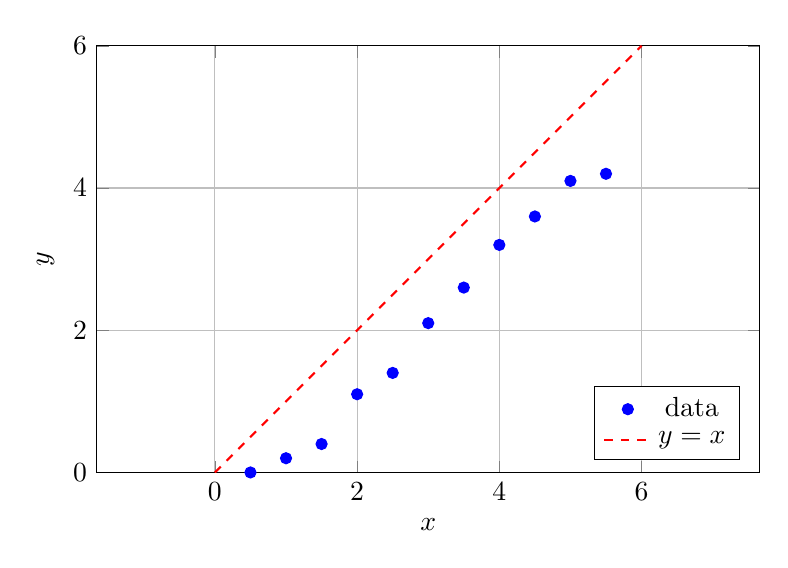
\begin{tikzpicture}
\begin{axis}[
    xlabel={$x$},
    ylabel={$y$},
    grid=both,
    width=10cm,
    height=7cm,
    axis equal,
    xmin=0, xmax=6,
    ymin=0, ymax=6,
    legend style={at={(0.97,0.03)}, anchor=south east},
]

% Scatter points roughly along the diagonal y = x
\addplot[
    only marks,
    mark=*,
    color=blue,
]
coordinates {
    (0.5,0.0)
    (1.0,0.2)
    (1.5,0.4)
    (2.0,1.1)
    (2.5,1.4)
    (3.0,2.1)
    (3.5,2.6)
    (4.0,3.2)
    (4.5,3.6)
    (5.0,4.1)
    (5.5,4.2)
};

% Add the diagonal reference line y = x
\addplot[
    domain=0:6,
    samples=2,
    thick,
    dashed,
    color=red,
]
{ x };
\addlegendentry{data}
\addlegendentry{$y = x$}

\end{axis}
\end{tikzpicture}
we assume that $S_\mathit{val}$ is identically distributed to $S_\mathit{test}$; however not independently.

    \item Describe conditions under which you’d expect $E_\mathit{test}[f_k ]$ and $E_\mathit{val} [f_k]$ to be nearly equal.


    The quantities $E_\mathit{test}[f_k]$ and $E_\mathit{val}[f_k]$ will be nearly equal when the following conditions hold:
    \begin{enumerate}[1.]
        \item $S_\mathit{val}$ is drawn \emph{independently and identically distributed} (i.i.d.) from the same distribution as $S_\mathit{test}$.
        \item The model selection or hyperparameter tuning does \emph{not} depend on $S_\mathit{test}$.
        \item The evaluation protocol (metrics, preprocessing, randomness) is consistent across both sets.
    \end{enumerate}
\end{enumerate}

\end{document}



